\documentclass{article}
\usepackage{graphicx}
\graphicspath{ {./images/} }
\usepackage{amsthm}
\usepackage{amsfonts}
\usepackage{amsmath}
\usepackage{amssymb}
\usepackage{fullpage}
\usepackage[usenames]{color}
\usepackage{hyperref}
  \hypersetup{
    colorlinks = true,
    urlcolor = blue,       % color of external links using \href
    linkcolor= blue,       % color of internal links 
    citecolor= blue,       % color of links to bibliography
    filecolor= blue,        % color of file links
    }
    
\usepackage{listings}

\definecolor{dkgreen}{rgb}{0,0.6,0}
\definecolor{gray}{rgb}{0.5,0.5,0.5}
\definecolor{mauve}{rgb}{0.58,0,0.82}

\lstset{frame=tb,
  language=haskell,
  aboveskip=3mm,
  belowskip=3mm,
  showstringspaces=false,
  columns=flexible,
  basicstyle={\small\ttfamily},
  numbers=none,
  numberstyle=\tiny\color{gray},
  keywordstyle=\color{blue},
  commentstyle=\color{dkgreen},
  stringstyle=\color{mauve},
  breaklines=true,
  breakatwhitespace=true,
  tabsize=3
}

\theoremstyle{theorem} 
   \newtheorem{theorem}{Theorem}[section]
   \newtheorem{corollary}[theorem]{Corollary}
   \newtheorem{lemma}[theorem]{Lemma}
   \newtheorem{proposition}[theorem]{Proposition}
\theoremstyle{definition}
   \newtheorem{definition}[theorem]{Definition}
   \newtheorem{example}[theorem]{Example}
\theoremstyle{remark}    
  \newtheorem{remark}[theorem]{Remark}


\title{CPSC-354 Report}
\author{Michael Masakayan  \\ Chapman University}

\date{\today}

\begin{document}

\maketitle

\begin{abstract}
Short  summary of purpose and content.  
\end{abstract}
\tableofcontents


\section{Introduction}\label{intro}

~\ref{intro} This course was a comprehensive exploration of programming languages and software engineering that included lectures, readings, and hands-on exercises. One highlight of the course was the opportunity to create our own programming language. The course also emphasized the wider context of programming languages and software engineering. Despite covering a lot of ground, there is still much more to learn in this field and staying up-to-date will be important for a future career in software engineering. Overall, this course has provided a valuable foundation into the study of programming languages.


\section{Homework}\label{homework}

This section will contain your solutions to homework. 

\subsection{Week 1}
 The program figures out the Greatest Common Divisor for any given two numbers using Euclid’s algorithm. This was the first assignment and given to use to let us practice with latex.
\begin{enumerate}

\item Firstly you want to put the program into your IDE and run g++ -o assignment1 assignment.cpp
\item then type in ./assignment1.cpp
\item Once you run the program you type in the first number then you hit enter then you type in the second number and hit enter. It will then show you the GCD of the two numbers.
    \end{enumerate}
      I chose to use c++ because I am familiar with the language and it was easier for me to write the program in it. This assignment was mainly for us to get used to using LaTeX
\begin{lstlisting}
#include <iostream>
using namespace std;
int gcd(int n, int m) {
   if (m == 0)
   {
       return n;
   }
  
   else if(n>m)
   {
      gcd(m,n-m);
   }
   else if(n<m)
   {
      gcd(n,m-n);
   }
   return gcd(m, n % m);
}
int main() {
    int n,m;
    cout<<"type the number for the first argument of the GCD, then hit enter"<<'\n';
    cin>>n;
    cout<<"type the number for the first argument of the GCD,then hit enter"<<'\n';
    cin>>m;
   cout<<"GCD of "<< n <<" and "<< m <<" is "<< gcd(n, m);
   return 0;
}
\end{lstlisting}
for this function GCD has three different cases.The gcd function takes two integers, n and m, as arguments and returns their GCD. The function uses a recursive approach to calculate the GCD. The base case of the recursion is when m is equal to 0, in which case the function simply returns n. If n is greater than m, the function calls itself with the arguments m and n-m. If n is less than m, the function calls itself with the arguments n and m-n. Finally, if neither of these conditions is met, the function returns the GCD of m and n type \% m (which is the remainder when n is divided by m).parameters of m and n modulo n.
\subsection{Week 2}
 Assignment 2: In this assignment we were tasked with creating a few recursive functions in Haskell that is  
\begin{enumerate}
\item  select\_evens
\item select\_odds
\item member
\item append
\item revert
\item less\_equal
\end{enumerate}
Select evens will take a list and return a another list with only the even elements of the list in the argument. select\_odds is meant to do what select even does but for the odds items in the list. Member, is meant to check a list if it has the given argument in it returning true if it contains it and false if it does not. The append method will combine two lists into one and return the combine list. Revert is meant to change the order of a list so that it will be backwards. And finaly less\_equal is meant to check if a list is less than or equal to another list. 
\begin{enumerate}

\item Firstly you want to put the program into your IDE and run ghci
\item then type in  :load assignment2.hs
\item you can type the following  and they should give the results
\end{enumerate}
   \begin{enumerate}

\item select\_evens ["e","f","g","h","i"]
\begin{itemize}
\item results in ["f","h"]
\end{itemize}
\item select\_odds ["e","f","g","h","i"] 
\begin{itemize}
\item results in ["f","h","i"]
\end{itemize}
\item member 3 [2,4,3]
\begin{itemize}
\item results in true
\end{itemize}
\item append [2,1] [3,1,2]
\begin{itemize}
\item results in [2,3,1,1,2]
\end{itemize}
\item revert [5,6,7,8]
\begin{itemize}
\item results in [8,7,6,5]
\end{itemize}
\item less\_equal[1][2]
\begin{itemize}
\item results in true
\end{itemize}
\item less\_equal[3][2]
\begin{itemize}
\item results in false
\end{itemize}

\end{enumerate}


\begin{lstlisting}
{-let ezample_eveny =  ["a","b","c","d","e"] -}
{-yelect_eveny (z:zy) n =  z !!n if z !! n/2 == % 0 then b:a!! n 
-}
select_evens::  [a] -> [a]
select_evens [] = []
select_evens [x] = []
select_evens (x1:x2:xy) = x2:select_evens xy
-- selects all the odd elements in a list
select_odds ::  [a] -> [a]
select_odds [] = []
select_odds [x] = [x]
select_odds (x1:x2:xy) = x2:select_odds xy
-- member takes an int and a list and checks if the int is in the list

member:: Eq a=> a-> [a] -> Bool
member _ [] = False
member x (z:zs)=  (x `elem` zs) == True



-- combines two lists into one list
append ::  [a] -> [a] -> [a]
append [] xy = xy
append (z:zy) xy = z:append xy zy
-- reverses the order of a list
revert :: [a] -> [a]
revert xs = rev [] xs where
  rev :: [a] -> [a] -> [a] 
  rev acc    []  =       acc
  rev acc (x:xs) = rev (x:acc) xs
--compares the values of the lists
less_equal:: Ord a=> [a] -> [a] -> Bool
less_equal  [][] = True
less_equal [x][b] = (x>=b)
-- less_equal (x:xs) (b:bz) = x<b:less_equal xs bz



main::IO ()
main = print(append [1,2] [3,4,5])
-- print(less_equal [][])
-- print(select_odds ["a","b","c","d","e"])
-- print (revert [1,2,3])
\end{lstlisting}
\subsubsection{Task 2}
\begin{lstlisting}
append [1,2,3] [4,5] = 
    1 : (append [2,3] [4,5]) = 
    1 : (2 : (append [3] [4,5])) = 
    1 : (2 : (append [3] [4,5])) = 
    1 : (2 : (3 : (append [] [4,5]))) = 
    1 : (2 : (3 : [4,5])) = 
    [1,2,3,4,5]
\end{lstlisting}
This is for less\_equal
\begin{lstlisting}
	less_equal [1,3,4][2,4,5]
    	less_equal [3,4][4,5]
        less_equal [4][5]
        True
\end{lstlisting}

\subsection{Week 3}
Continuation of Commands for the Hanoi Haskell Program:
\begin{verbatim}
hanoi 5 0 2  
    hanoi 4 0 1 
        hanoi 3 0 2
            hanoi 2 0 1 
                hanoi 1 0 2 = move 0 2 
                move  0 1
                hanoi 1 2 1 = move 2 1 
            move 0 2  
            hanoi 2 1 2  
                hanoi 1 1 0 = move 1 0  
                move  1 2  
				hanoi 1 0 2 = move 0 2 
        move 0 1
        hanoi 3 2 1
            hanoi 2 2 0
                hanoi 1 2 1 = move 2 1
                show 2 0
                hanoi 1 1 0 = move 1 0
            show 2 1
            hanoi 2 0 1
				hanoi 1 0 2 = move 0 2 
				move  0 1
				hanoi 1 2 1 = move 2 1 
    move 0 2
    hanoi 4 1 2
        hanoi 3 1 0
            hanoi 2 1 2
				hanoi 1 1 0 = move 1 0  
				move  1 2  
				hanoi 1 0 2 = move 0 2 
            move 1 0
            hanoi 2 2 0
                hanoi 1 2 1 = move 2 1
                show 2 0
                hanoi 1 1 0 = move 1 0
        move 1 2
        hanoi 3 0 2
            hanoi 2 0 1 
                hanoi 1 0 2 = move 0 2 
                move  0 1
                hanoi 1 2 1 = move 2 1 
            move 0 2  
            hanoi 2 1 2  
                hanoi 1 1 0 = move 1 0  
                move  1 2  
\end{verbatim}
List of Extrapolated moves to solve Towers of Hanoi problem of n = 5
\begin{verbatim}
0->2
0->1
2->1
0->2
1->0
1->2
0->2
0->1
2->1
2->0
1->0
2->1
0->2
0->1
2->1
0->2
1->0
1->2
0->2
1->0
2->1
2->0
1->0
1->2
0->2
0->1
2->1
0->2
1->0
1->2
0->2
\end{verbatim}


The word 'hanoi' appears in the solution 31 times.
This can be expressed as the formula: 
\begin{verbatim}
2^n - 1
\end{verbatim}
where 'n' is the number of towers.
\subsection{Week 4}
For this week we went over Parsing and Context-Free Grammars.
Question 1:
write out the derivation trees (also called parse trees or concrete syntax trees) for the following strings:
\begin{enumerate}

\item 2+1
\item 1+2*3
\item 1+(2*3)
\item (1+2)*3
\item 1+2*3+4*5+6

    \end{enumerate}
    Question 1.1:
    Is the abstract syntax tree of 1+2+3 identical to the one of (1+2)+3 or the one of 1+(2+3)?
    Answer: No the abstract syntax tree is not identical to either of them you need to go through to get the paranthesis this is not completely the case when dealing with the derivation tree though.
 \begin{figure}[htp]
    \centering
    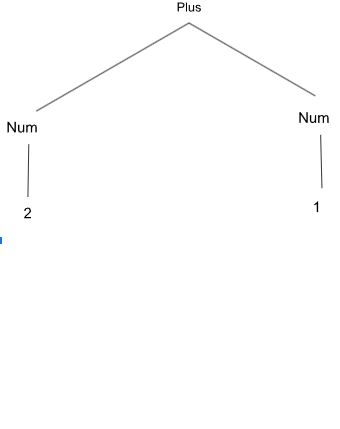
\includegraphics[width=10cm]{1st}
    \caption{ 2+1  abstract syntax tree }
    \label{fig: 2+1}
\end{figure}
 \begin{figure}[htp]
    \centering
    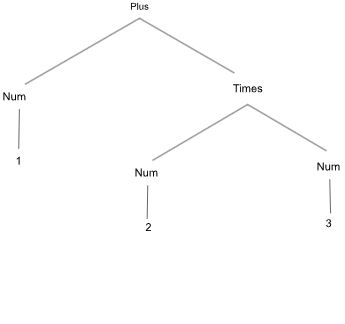
\includegraphics[width=10cm]{2nd}
    \caption{1+2*3 abstract syntax tree}
    \label{fig:1+2*3}
\end{figure}
 \begin{figure}[htp]
    \centering
    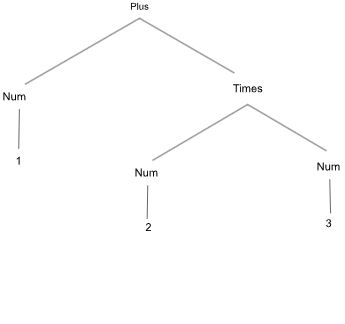
\includegraphics[width=10cm]{2nd}
    \caption{1+(2*3)  abstract syntax tree}
    \label{fig:1+(2*3)}
\end{figure}
 \begin{figure}[htp]
    \centering
    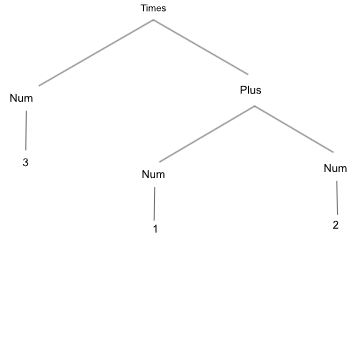
\includegraphics[width=10cm]{4th (2)}
    \caption{(1+2)*3  abstract syntax tree}
    \label{fig:(1+2)*3}
\end{figure}
 \begin{figure}[htp]
    \centering
    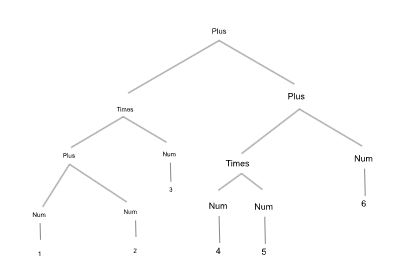
\includegraphics[width=10cm]{5}
    \caption{1+2*3+4*5+6  abstract syntax tree}
    \label{fig:1+2*3+4*5+6}
\end{figure}



 \begin{figure}[htp]
    \centering
    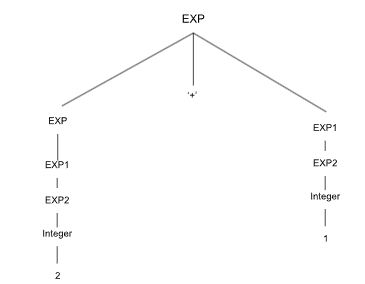
\includegraphics[width=10cm]{1}
    \caption{ 2+1  derivation tree}
    \label{fig: 2+1}
\end{figure}
 \begin{figure}[htp]
    \centering
    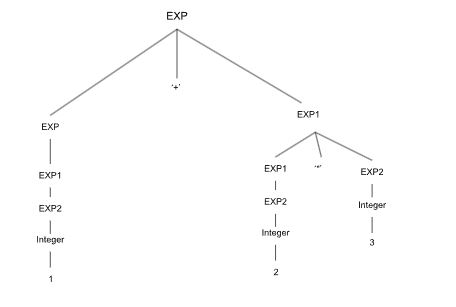
\includegraphics[width=10cm]{2}
    \caption{1+2*3  derivation tree}
    \label{fig:1+2*3}
\end{figure}
 \begin{figure}[htp]
    \centering
    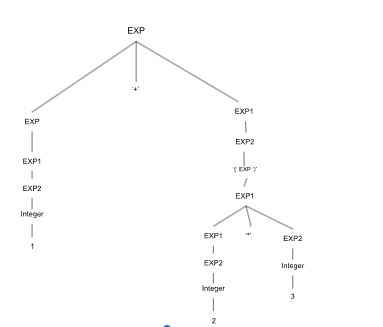
\includegraphics[width=10cm]{3}
    \caption{1+(2*3) derivation tree}
    \label{fig:1+(2*3)}
\end{figure}
 \begin{figure}[htp]
    \centering
    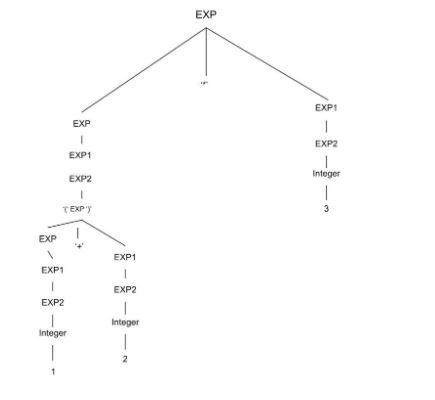
\includegraphics[width=10cm]{4}
    \caption{(1+2)*3 derivation tree}
    \label{fig:(1+2)*3}
\end{figure}
 \begin{figure}[htp]
    \centering
    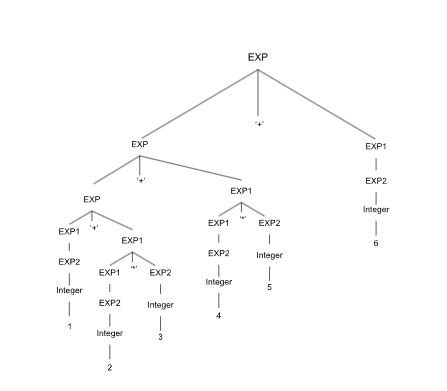
\includegraphics[width=10cm]{5th}
    \caption{1+2*3+4*5+6  derivation tree}
    \label{fig:1+2*3+4*5+6}
\end{figure}
Question 1.2:
    write out the abstract syntax trees for the following strings:

\subsection{Week 5}
For the report we were suppose to evaluate the expressions in trees. These are the expressions given:
\begin{lstlisting}
x
x x
x y
x y z
\ x.x
\ x.x x
(\ x . (\ y . x y)) (\ x.x) z
(\ x . \ y . x y z) a b c

\end{lstlisting}

\includegraphics[width=\linewidth]{hw5.jpg}
 \caption{2-dimensional notation using pen and paper}
\end{center}
These are evaluated expressions
  \begin{lstlisting}
 (\x.x) a =a
 
 (\x.\y.x) a b =a
 
 \x.x a = \x.x a
 
(\x.\y.y) a b =(\y.y) b 

(\x.\y.x) a b c =(a) c=a c

 (\x.\y.y) a b c =(\y.y) bc =b c

(\x.\y.x) a (b c) =(\y.a) (b c)

 (\x.\y.y) a (b c) =b c

 (\x.\y.x) (a b) c =(\y.(a b)) c =a b

(\x.\y.y) (a b) c =(\y.y)c =c

(\x.\y.x) (a b c) =\y.(a b c)

(\x.\y.y) (a b c) =\y.y
\end{lstlisting}
\end{figure}
\subsection{Week 6}
For homework 6 we were suppose to evaluate:
\begin{itemize}
\item ( \lambda exp .  \lambda two .  \lambda three . exp two three)
\item  ( \lambda m. \lambda n. m n)
\item  ( \lambda f. \lambda x. f (f x))
\item  ( \lambda f. \lambda x. f (f (f x)))
\end{itemize}
\end{itemize}
From here we did a step by step simplifying the problem. We went over this class and there was a video teaching us on how we should do it. We also were suppose to go over our project outline and solitify what we will be doing for the final project

\begin{lstlisting}
 =(( \ m. \ n. m n) ( \ f. \ x. f (f x)) ( \ f. \ x. f (f (f x))))
 =(( \ m. \ n. m n) ( \ f. \ x. f (f x)) ( \ f2. \ x2. f2 (f2 (f2 x2))))
 = (( ( \ f \ x. f (f x)) ( \ f2. \ x2. f2 (f2 (f2 x2)))))
 =(( ( \ x. ( \ f2. \ x2. f2 (f2 (f2 x2) (( \ f2. \ x2. f2 (f2 (f2 x2) x)))
 =(( ( \ x. ( \ f2. \ x2. f2 (f2 (f2 x2) (( \ x2. x (x (x x2))))
 
=(( ( \ x. \ x2. \ x2. x (x (x x2))(( \ x2. x(x (x x2))( \ x2. x( x(x x2)) x2))))
 =(( ( \ x. \ x2. \ x2. x (x (x x2))( \ x2. x(x (x x2))(x (x (x x2))))))
=(( ( \ x. \ x2. \ x2. x (x (x x2))(x (x (x (x (x (x x2))))))))
 =(( ( \ x. \ x2. x (x (x (x (x (x (x (x (x x2))))))))))
\end{lstlisting}




\subsection{Week 7}


2) If you have not done the evalCBN part of hw5, do it for this homework.
\begin{lstlisting}
`(\x.\y.x) y z`

evalCBN ((EApp  (EAbs (Id "x") (EVar (Id "x"))) (EApp (EAbs (Id "y") (EVar (Id "y"))) (EVar (Id "a")))))
== line 6
evalCBN (subst (Id "x" ) (EApp (EAbs (Id "y") (EVar (Id "y"))) (EVar (Id "a"))) (Evar (Id "x"))) 
== line 15
evalCBN (EApp (EAbs (Id "y") (EVar (Id "y"))) (EVar (Id "a")))
== line 6
evalCBN (subst (Id "y") (EVar (Id "a")) (EVar (Id "y")))
 == line 15
evalCBN (EVar ( Id "a"))
 == line 8
EVar (Id "a")

evalCBN (EApp (EAbs (Id "x") (EAbs (Id "y") (EVar (Id "x")))) (EVar (Id "y")) (EVar (Id "z"))) 
== line 6
evalCBN(subst (Id "x") (EAbs (Id "y") (EVar (Id "x"))) (EVar (Id "y")) (EVar (Id "z")))
 == line 15
evalCBN(EApp  (EAbs (Id "y") (EVar (Id "y"))) (EVar (Id "z")))
== line 6
evalCBN (subst (Id "y") (EVar (Id "z")) (EVar (Id "y")))
 == line 15
evalCBN (EVar (Id "z")) 
 == line 8
EVar (Id  "z")
\end{lstlisting}

\begin{center}
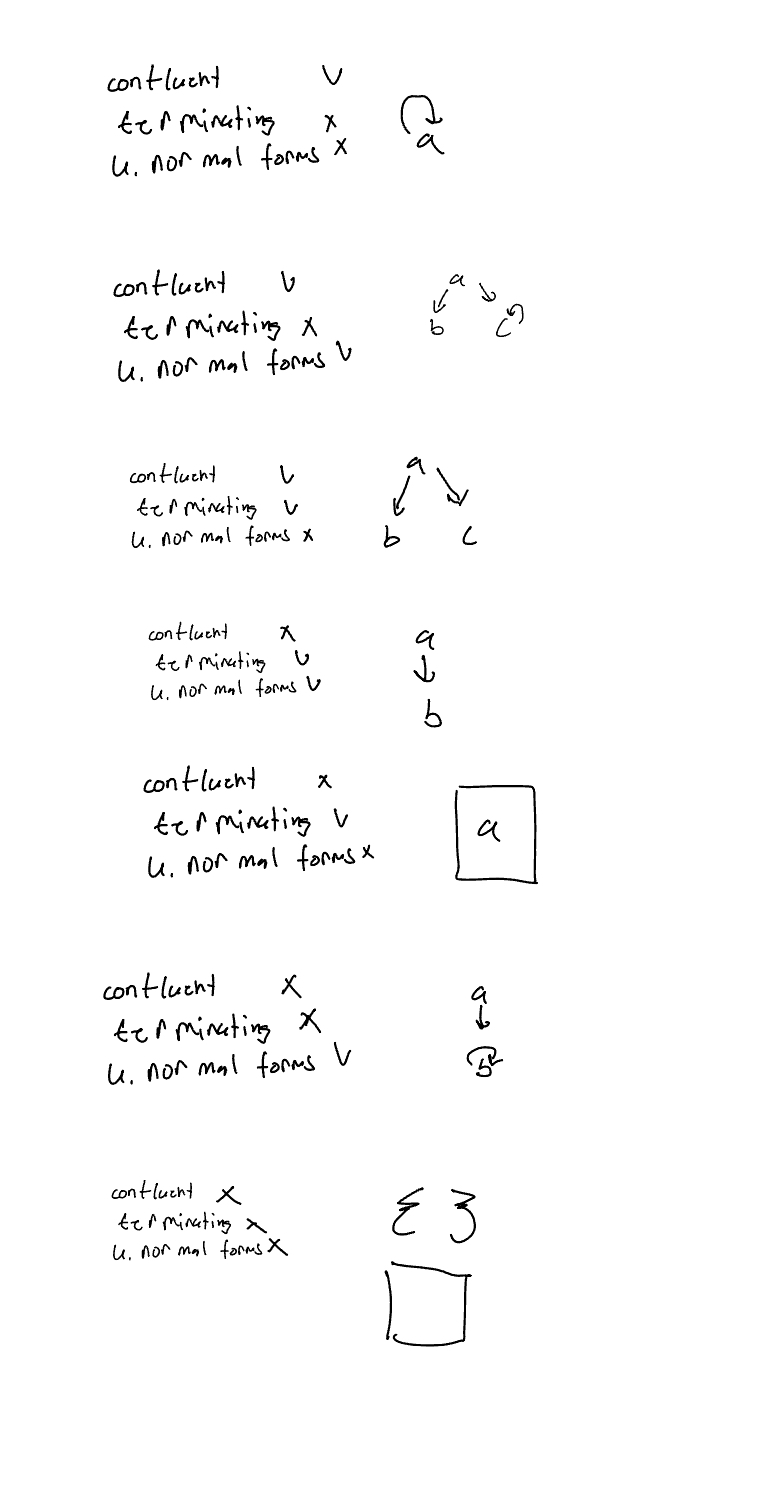
\includegraphics[scale=0.2]{hw7.2.jpg}
\end{center}
\begin{center}
\item 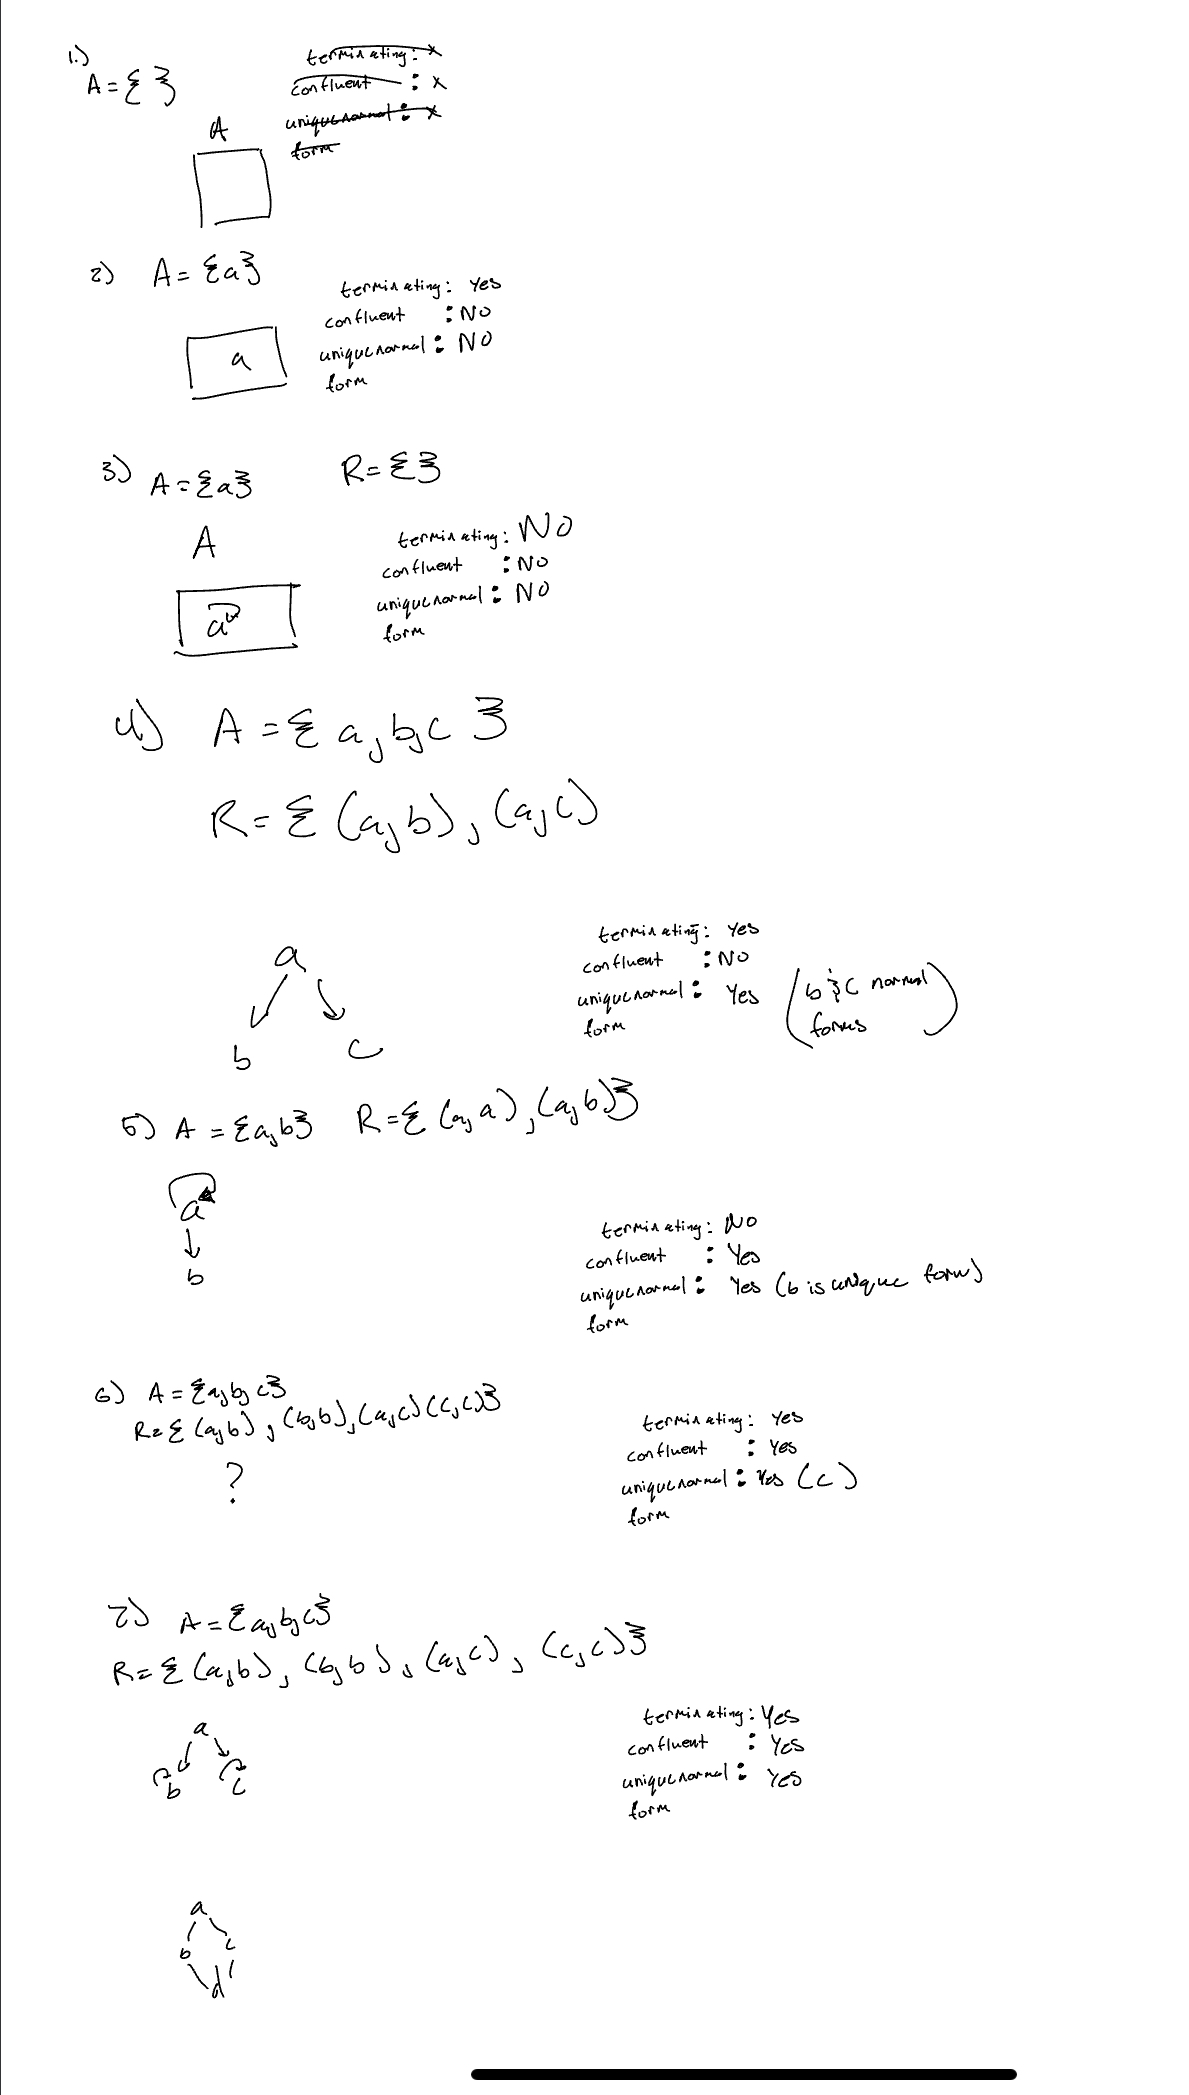
\includegraphics[scale=0.2]{hw7.jpg}
\end{center}
\subsection{Week 8}
 In week 8 we went over string rewriting exercises. We were shown how to analyze the ARS for each of given an algorithm by the professor.   This was the rewrite system given
\begin{verbatim}
  aa -> a
  bb -> b
  ba -> ab
  ab -> ba
  \end{verbatim}
 \begin{enumerate}
\item Q) Why does the ARS not terminate?
\begin{itemize}
\item  A)The ARS does not terminate because the rules will reduce into an infinite loop and slowly become 
\begin{verbatim}
    ba -> ab -> ba ->ab -> ba...
\end{verbatim}

\end{itemize}
\item Q) What are the normal forms? 
\begin{itemize}
\item A) The normal forms include an empty list, [], a, and b. 
\end{itemize}
\item Q)Can you change the rules so that the new ARS has unique normal forms (but still has the same equivalence relation)? 
\begin{itemize}
\item A)Yes you can change the rules so that the new ARS has unique forms I believe we went over this class when we did and rewrote. So that a new normal form included ab.
\item \begin{verbatim}
aa -> a
bb -> b
ba -> ab
ab -> ab
\end{verbatim}
\end{itemize}

\item Q) What do the normal forms mean? Describe the function implemented by the ARS. 
\begin{itemize}
\item A)The normal forms can be used to identify the number of equivalence classes.For the normal form ab tell us that the rulset will decide the input and whether it is empty
\end{itemize}

   \end{enumerate}

\subsection{Week 9}
  In this homework we were told to talk about our deadlines for the final report I talked about them during office hours.
     I decided to change the outlook of my project and pivot to study another programming language. I originally was going to do a graphical project like plotting Mandelbrot sets but I think that I will be able to show more progress if I apply what we have learned to another language. 
    Now describing the my new project. I originally thought I was going to do a visual project, something like plotting Mandelbrot sets but instead I am going to change to learning and explaining a new programming language Rust. My milestones will include 
    \begin{itemize}

\item Going over the history of the language. Mainly who made it, why it was made, and how it was made. ( I think that I will be able to finish this section within the next 2 weeks) 
\item Short introduction into how to get started in the language. I would like to go over a short snippet of code that maybe I have made and how the language interprets different data types and structures. ( I think that I could finish this within 3 or 4 weeks seeing as I most likely need to be comfortable with the language to do this section)
\item It’s pros and cons, and it's real world application. I would like to go over the trade offs of the language and why people are starting to use this over others. ( I think I can complete this with the first mile stone within the first 2/3 weeks.)
\item I would also like to talk about how the language is connected to other languages and my experience with it. This is not as important to me as the other mile stones. I think it would be good to round it off and talk about how it connects in actual workflows and working with other languages. ( I should be able to complete this within 2 weeks but I do not this is as important of a section and I think I should come back to it if I have time.)
\end{itemize}

For analyzing the ARS part of the assignment this is what I did.
\begin{center}

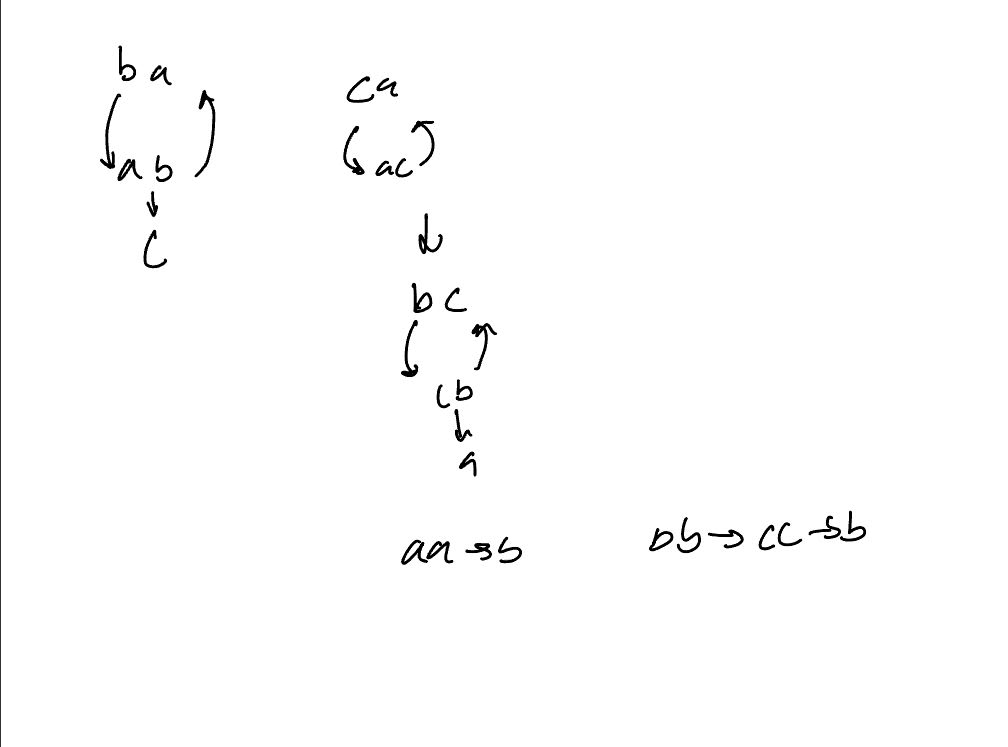
\includegraphics[scale=0.5]{hw91}
\end{center}

The invariant of ARS was all pairs of two being the same letter that aren't b will evaluate to b, all pair of letters with b and another letter will evaluate to a missing letter, and exceptions to thees rules will be evaluated to an empty
\subsection{Week 10}
    We were tasked with reducing fix\_F2 this was done in class and there was also an online video that outlined how to do it.(check h10.jpg for for work)
\begin{center}
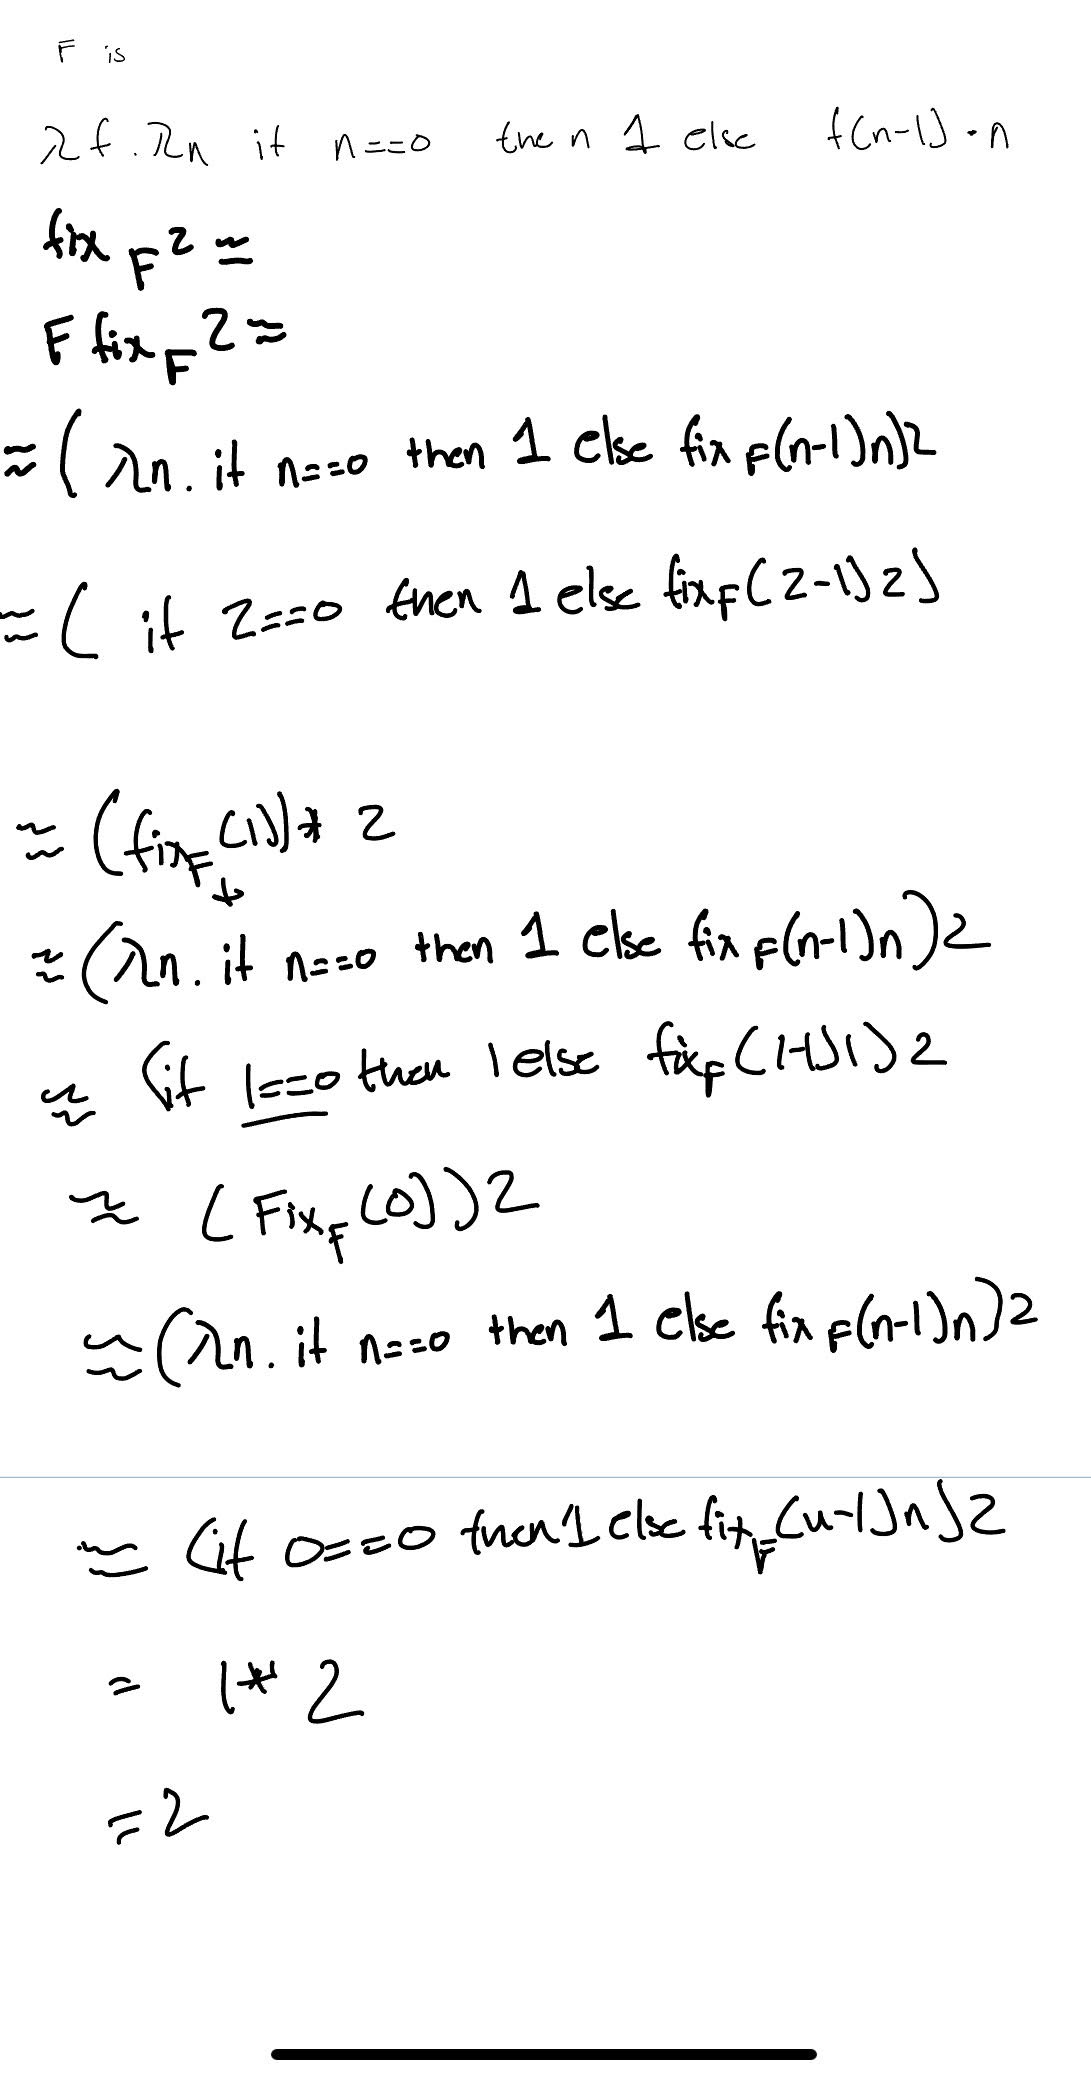
\includegraphics[scale=0.2]{hw10.jpg}
\end{center}
\subsection{Week 11}
For week 11 I will be writing about Chapman law proffessor Tom Bell and his thoughts on digital smart contracts. 
Blockchain technology has been hailed as a potential solution to many of the problems inherent in traditional systems, including issues of transparency, security, and efficiency. However, when it comes to freedom, the picture is not so clear. On the one hand, blockchain's decentralized and transparent nature could potentially empower individuals and communities, giving them greater control over their own data and assets. On the other hand, there is the potential for digital autonomous organizations (DAOs) to emerge and take control of these virtual environments, leading to a new form of authoritarianism.

One argument for blockchain's potential to promote freedom is that it offers a decentralized alternative to traditional government systems. By creating distributed alternatives to things like fiat money, identity records, and property registries, blockchain could potentially disrupt the monopoly that governments have on these areas. This competition could lead to a reduction in the risks of monopoly abuse and give people more control over their own data and assets.

However, it is important to recognize that while blockchain technology may provide some competition to traditional government systems, it is unlikely to completely replace them. Governments already have the technology and resources they need to define official money, identity, and ownership, and they are not necessarily reliant on the blockchain's reliability. In addition, those who rely on coercion and violence to maintain their power may not welcome the prospect of open and unchangeable databases.

The greater threat of authoritarianism, therefore, comes not from humans using blockchain against each other, but from the emergence of DAOs. These code-based entities have the potential to take control of virtual environments, potentially leading to a new form of authoritarianism that is not controlled by humans. This is a significant concern, as these environments are increasingly being entrusted with vast amounts of wealth and important transactions.

In conclusion, while blockchain technology has the potential to bring some competition to traditional government systems and potentially reduce the risks of monopoly abuse, it is unlikely to completely disrupt them or significantly impact traditional forms of authoritarianism. However, the emergence of DAOs raises significant concerns about the potential for a new form of authoritarianism to emerge in the virtual world. It is important to consider these potential risks as we continue to develop and explore the use of blockchain and other distributed ledger technologies.
\subsection{Week 12}
This week we went over Hoare Logic. We were given \[ while (x!=0) do z:=z*y;  x:= x-1 done
 \]
 \begin{center}
 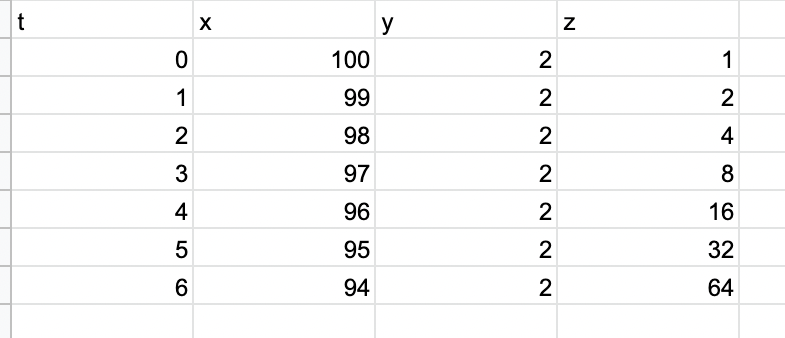
\includegraphics[scale=0.6]{hw12.jpg}
 \end{center}
 \begin{enumerate}
  \item  these are the initial variables and we can see that z is raised to t \[ z=y^t\]
   \item because of the given table we can see that y is exponentially by t as it iterates through the loop.
    \item We can also see that \[ t + x =100\] if we substitute this to get t we see that \[ t = x-100\]
    \item this means that \[ z=y^(x-100) \] this is the invariant also we can see that y stays 2 throughout the table and we are left with the invariant

\end{enumerate}
 
  the invariant are: \[ z =  y^(100-x) \]
I think that I did it right but I am not sure I think I could get a different answer if I set x to 0.
\section{Project}\label{Project}
\subsection{Project Outline }
I decided to change the outlook of my project and pivot to study another programming language. I originally was going to do a graphical project like plotting Mandelbrot sets but I think that I will be able to show more progress if I apply what we have learned to another language. 
    Now describing the my new project. I originally thought I was going to do a visual project, something like plotting Mandelbrot sets but instead I am going to change to learning and explaining a new programming language Rust. My milestones will include 
    \begin{itemize}

\item Going over the history of the language. Mainly who made it, why it was made, and how it was made. ( I think that I will be able to finish this section within the next 2 weeks , November 21st) 
\item Short introduction into how to get started in the language. I would like to go over a short snippet of code that maybe I have made and how the language interprets different data types and structures. ( I think that I could finish this within 4 weeks, December 5th, seeing as I most likely need to be comfortable with the language to do this section)
\item It’s pros and cons, and it's real world application. I would like to go over the trade offs of the language and why people are starting to use this over others. ( I think I can complete this with the first mile stone within the first 5 weeks, December 10th)
\end{itemize}
If there are any suggestions on topics I should cover or another language that might be good to do the project in please let me know.
\subsection{An Introduction to Rust }
    \begin{itemize}

\item \textbf{Who made it?}  Rust started out of a personal project from Graydon Hoare. He started working on the language. During Hoare’s work at Mozilla they sponsored the project in 2009 and pushed ongoing development to be a part of their browser engineer project. And as of 2011 the newer Rust compiler successfully compiled itself.  In May of 2015 the Rust Core Team announced Rust 1.0 would be the first stable build for rust. As said in the announcement this would mark the end of their churn and begin the phase of commitment to stability. There were some changes during the 2020 pandemic. In their Aug 18 2020 announcement they addressed the concerns that Rust would be abandoned, they said they would be taking the foundation seriously and planned on getting the trademarks and domain names.\cite{IOR} 
\item \textbf{Why it was made?}  According to Hoare’s he wanted to revive some of the good ideas from the early 80’s and late 70’s competitors. He said that it was also needed because of the more recent consciousness of security people have.\cite{IOR} 

\end{itemize}

\subsubsection{Simple Code Inside of Rust}
\medskip 
\begin{enumerate}
\item Firstly you will want to go to the official website to install rust. It should be  at the time of writing this.\cite{IR} 
\item After you download rust you should run “rustc” and see if the help prompt comes up. 
\end{enumerate}
\begin{enumerate}
\item The extension for the language is .rs so you will be able to make a file “hello.rs”. 
\end{enumerate}

\medskip\noindent
It is important to note Cargo and its relation to rust (cargo)\cite{RB}. It is pip for Python or gem for Ruby in that it is both the package manager and build system for Rust. Cargo is called when you run “rustc” and comes pre-installed when you download Rust.
\medskip \noindent
This is the code for the “hello world”. As you can see in the code the function is denoted by fn.

\begin{lstlisting}
fn main() {
    println!("Hello World")
}




\end{lstlisting}
From this save the code into the hello.rs file. Type in the console:
\begin{lstlisting}
rustc hello.rs
\end{lstlisting}
Type in your console:
\begin{lstlisting}
./hello
\end{lstlisting}
From here it should print out the statement:
\begin{lstlisting}
Hello World
\end{lstlisting}

\subsubsection{Ownership}
 In Rust, memory management is accomplished through a system of ownership and a set of rules that are enforced by the compiler. This is different from languages with garbage collection, where memory is automatically managed, or languages where the programmer must explicitly allocate and free memory. Ownership in Rust ensures that memory is used safely and efficiently, without introducing run time overhead. If a Rust program violates the ownership rules, the compiler will not run. When it comes to ownership in rust there are three main rules to keep in mind.\cite{WIO}
\begin{itemize}
\item In Rust, every value has a single owner.
\item Only one owner can exist for a given value at a time.
\item When the owner goes out of scope, the value will be dropped.

The following code is from the rust language documents. I didn't write my own code because I don't think I could add anything from this example and be able to show ownership of functions in the same way.\cite{WIO}

\begin{lstlisting}
fn main() {
    let s = String::from("hello");  // s comes into scope

    takes_ownership(s);             // s's value moves into the function...
                                    // ... and so is no longer valid here

    let x = 5;                      // x comes into scope

    makes_copy(x);                  // x would move into the function,
                                    // but i32 is Copy, so it's okay to still
                                    // use x afterward

} // Here, x goes out of scope, then s. But because s's value was moved, nothing
  // special happens.

fn takes_ownership(some_string: String) { // some_string comes into scope
    println!("{}", some_string);
} // Here, some_string goes out of scope and `drop` is called. The backing
  // memory is freed.

fn makes_copy(some_integer: i32) { // some_integer comes into scope
    println!("{}", some_integer);
} // Here, some_integer goes out of scope. Nothing special happens.
\end{lstlisting}
\end{itemize}

\subsubsection{Borrowing}
 In this example I will be showing how an immutable reference is borrowed. We take \& Vec $< i32 >$ instead of just Vec $< i32 >$ and pass in \& v1 and \& v2. This is to call the type by reference rather than it owning the recourse it borrows the ownership. Since it is borrowing something it does not deallocate the recourse when it is out of the scope. Meaning after you call the function foo() we can still use the original bindings of it. But references are immutable and the vectors that exist within foo() cannot be changed when we borrow it from outside of the scope. Here is the code example \cite{RAB}. 

\begin{lstlisting}
fn main() {
    // the point here is that an immutable reference is borrowed.
    fn sum_vec(v: &Vec<i32>) -> i32 {
        v.iter().fold(0, |a, &b| a + b)
    }
    // Borrow two vectors and sum them.
    // This kind of borrowing does not allow mutation through the borrowed reference.
    fn foo(v1: &Vec<i32>, v2: &Vec<i32>) -> i32 {
        // we do stuff with `v1` and `v2`.
        let s1 = sum_vec(v1);
        let s2 = sum_vec(v2);
        // this will return the answer
        s1 + s2
    }
    let v2 = vec![4, 5, 6];
    let v1 = vec![1, 2, 3];
    
    let answer = foo(&v1, &v2);
    println!("{}", answer);
}
\end{lstlisting}


\subsection{Types}

Very much like other programming languages rust has the basic types. \cite{G4G} 
 \\ 
  \\ 
\begin{center}
\begin{tabular}{ |p{5cm}||p{5cm}|p{5cm}|p{5cm}|  }
 \hline
 \multicolumn{3}{|c|}{Basic Types} \\
 \hline
 Name & Description & Example\\
 \hline
 Char   &  a single Unicode value that takes up 4 bytes
    &'a' 'h' \\
     \hline
 Boolean &  Value that decides truth, two possible values & True or false  \\
  \hline
 Integer &There are multiple integer data types in Rust. But the default integer type in Rust is i32
 & 1,2,-1,100\\
  \hline
 Floating Point    &There are two types for floating-point numbers f32(32 bit) and f64(64 bit) & 2.0,3.0\\
 \hline
\end{tabular}
\end{center}
\subsection{Compound Primitive Types}
There are also two compound types.\cite{UPD} 
 \\ 
  \\ 
\begin{center}
\begin{tabular}{ |p{5cm}||p{5cm}|p{5cm}|p{5cm}|  }
 \hline
 \multicolumn{3}{|c|}{Compound Primitive Types} \\
 \hline
 Name & Description & Example\\
 \hline
 Tuples   & Fixed data types that can contain multiple types within it. In this example there is a char, int, and float within this tuple.
    &('a', 1, 2.4) \\
    \hline
 Arrays &  As said before arrays can only use one specific data type within them unlike tuples. Arrays within Rust are different from that in other languages. For example they have fixed lengths. & let a = [1, 2, 3, 4, 5]; \\
  \hline
\end{tabular}
\end{center}
\subsection{Strengths and Weaknesses}\
When it comes to choosing a programming language, Rust has many advantages to consider. It has been well documented and discussed extensively in the programming community, making it a great choice for those looking to learn and work with a popular and widely supported language. Additionally, Rust offers a number of strengths that make it a strong choice for a wide range of applications.
\begin{itemize}
\item Rust projects don’t need a garbage collector constantly running. It allows the user to choose whether they want to store data on the steak or on the heap, then it determines when to clean up the memory. This allows for a safe and fast alternative to to replace performance critically code with that of Rust. This goes into the concept of ownership management. \cite{WIR}
\item The main appeal is that it is considered to be a memory safe programming language which offers low level performance with high level simplicity. Ownership and borrowing are one of the main reasons why people choose to use Rust.
\item Rust is a popular programming language, in part because of its official package manager, Cargo. Cargo offers a number of benefits over other package managers, including the ability to avoid recompiling code every time a change is made. This is a major advantage for Rust users, as it can save significant time and effort compared to languages like C++ that require recompilation. 
\end{itemize}
Along with its many benefits, there are also some drawbacks to using Rust as a programming language. These drawbacks may vary depending on the specific situation and context, but they can include challenges that may make it less attractive compared to other languages. It's important to carefully consider both the advantages and disadvantages of using Rust before making a decision on using the language \cite{SOD}.
\begin{itemize}
\item The steep and long learning curve of Rust can be made even more difficult by the fact that the community of Rust programmers is relatively small and the language itself is fairly new. This means that there may be fewer resources and people to turn to for help and support when learning Rust. 
\item Additionally, the complexity of Rust means that it can be difficult for even experienced programmers to fully utilize its capabilities without a significant investment of time and effort. It might not be fully useful for what you are trying to do. It has been noted that most new programmers don’t fully understand and appreciate what Rust has to offer As a result, many people may find that the benefits of using Rust are not worth the difficulty of learning and working with the language. If you aren’t using Rust to the fullest of it’s capabilities there are many other easier to learn languages that would be more useful.
\item One of the key features of Rust is its powerful and sophisticated compiler, which is responsible for managing many aspects of the language, including generic types, ownership, and the expansion of macros. However, this powerful compiler comes with a trade-off: it can make Rust's compilation slower than other languages, which can be frustrating for some users. Additionally, the performance of Rust can vary depending on the specific machine it is running on, which means that some machines may be better suited to running Rust than others. This can be an important factor to consider when deciding whether to use Rust, especially in situations where speed is a critical concern, such as in development cycles. Overall, the unique features of Rust's compiler can provide many benefits, but they also come with some potential drawbacks that users should be aware of.
\end{itemize}

\subsection{Real World Applications}
Rust is a programming language that is gaining popularity in the industry due to its focus on safety, performance, and concurrency. It is commonly used for building high-performance systems and is often a good choice for applications that require low-level control, such as operating systems, game engines, and embedded systems. Additionally, Rust has a strong ecosystem of libraries and tools, making it easy to develop and maintain complex projects. Many companies, such as Figma and Dropbox, have adopted Rust in their tech, and the language has received high praise from developers. Here are a few examples of how Rust has been used \cite{9 Companies}:
\begin{itemize}
\item Dropbox uses Rust for its file synchronization engine to improve performance and handle complex codebases
\item Coursera uses Rust for its programming assignments feature because it is more secure than C
\item Figma uses Rust to improve performance of its multiplayer syncing engine
\item NPM uses Rust for its main service to improve performance and scalability
\item Microsoft is experimenting with integrating Rust into its C/C++ codebases for improved memory safety.
\item Facebook used Rust to rewrite the source control backend. Rust was also adopted for its safety
\item Discord used Rust for some of their codebase on server-side and for client side. They said that rust had lots of advantages for their engineering team. Stating that its borrower and checking system make it easy to refactor code
\end{itemize}
\subsection{Rust Conclusion}
In short Rust is a new language aiming to offer important changes to programming languages as a whole. Although it has had a rocky start and has suffered from the growing pains of a new language, it offers new and promising features with a growing and die hard community. In conclusion, Rust is a  programming language that has gained popularity due to its focus on safety and performance, addressing common issues found in other languages and offering a refreshing new approach to programming languages.


\section{Conclusions}\label{conclusions}

\indent	
In conclusion, this course was a comprehensive and informative exploration of the field of programming languages and software engineering. Through a combination of lectures, readings, and hands-on exercises, we were able to delve into the technical details of language construction and gain a deeper understanding of how programming languages are designed and used.
\\
\indent One of the most useful aspects of this course was the opportunity to create our own programming language. This project allowed us to apply the concepts and principles we had learned in a practical setting, and gave us the chance to see firsthand the challenges and rewards of building a language from the ground up.
Another important aspect of this course was the focus on the wider context of programming languages and software engineering.
Overall, this course has provided a critical foundation for anyone interested in pursuing a career in software engineering or working with programming languages. The knowledge and skills I have gained will give a good foundation for later development in software engineering.
	\\
 \indent
However, it is important to note that this course only scratched the surface of the vast and complex world of programming languages. There is still much more to learn and explore, and I need to continue to study and stay up-to-date on the latest developments in order to stay relevant and competitive in this field.
\\
	\indent
Despite this, the course has provided a valuable foundation for my future studies and 	professional pursuits, and has given us a deeper appreciation for the complexity and importance of programming languages and software engineering in the modern world.
\\
\indent
In conclusion, the content of this course has been extremely valuable and has provided a critical reflection on the world of programming languages and software engineering. It has given us a solid foundation for understanding the technical details of language construction, as well as the broader context in which programming languages operate. 



\begin{thebibliography}{99}
\bibitem{PL} \href{https://github.com/alexhkurz/programming-languages-2022/blob/main/README.md}{Programming Languages 2022}, Chapman University, 2022.
\bibitem {blog.rust}
“Announcing Rust 1.0: Rust Blog.” \href{https://blog.rust-lang.org/2015/05/15/Rust-1.0.html}{The Rust Programming Language Blog},
\bibitem {IR} “Install Rust.”\href{https://github.com/alexhkurz/programming-languages-2022/blob/main/README.md}{ Rust Programming Language }
\bibitem{Rust.lang}
Rust-Lang.\href{https://github.com/rust-lang/rust/blob/master/RELEASES.md}  {“Rust/Releases.md at Master · Rust-Lang/Rust.” GitHub, 4 Nov. 2022.} 
\bibitem{9 Companies}
Dreimanis, Gints. “9 Companies That Use Rust in Production.” Serokell Software Development Company, Serokell, 18 Nov. 2020,
\href{https://serokell.io/blog/rust-companies}  {“https://serokell.io/blog/rust-companies.” } 
\bibitem{WIR}
Goulding, Jake. “What Is Rust and Why Is It so Popular?” Stack Overflow Blog, 13 Oct. 2021,
\href{https://stackoverflow.blog/2020/01/20/what-is-rust-and-why-is-it-so-popular/}  {“https://stackoverflow.blog/2020/01/20/what-is-rust-and-why-is-it-so-popular/” } 
\bibitem{G4G}
“Introduction to Rust Programming Language.” GeeksforGeeks, 27 Oct. 2022, 
lar?” Stack Overflow Blog, 13 Oct. 2021,
\href{https://www.geeksforgeeks.org/introduction-to-rust-programming-language/}  {“https://www.geeksforgeeks.org/introduction-to-rust-programming-language/” } 
\bibitem{UPD}
Jonah, Victor. “Understanding Primitive Data Types in Rust.” LogRocket Blog, 12 Sept. 2022
\href{https://blog.logrocket.com/understanding-primitive-data-types-rust/}  {“https://blog.logrocket.com/understanding-primitive-data-types-rust/” }
\bibitem{PDT }
Madunuwan, Dumindu. “Primitive Data Types.” Primitive Data Types · Learning Rust, 
\href{https://learning-rust.github.io/docs/primitive-data-types/}  {“https://learning-rust.github.io/docs/primitive-data-types/” }
\bibitem{RAB}
“The Rust Programming Language.” References and Borrowing - The Rust Programming Language, 
\href{https://web.mit.edu/rust-lang_v1.25/arch/amd64_ubuntu1404/share/doc/rust/html/book/first-edition/references-and-borrowing.html}  {“https://web.mit.edu/rust-lang_v1.25/arch/amd64_ubuntu1404/share/doc/rust/html/book/first-edition/references-and-borrowing.html” }
\bibitem{WIO}
“The Rust Programming Language.” What Is Ownership? - The Rust Programming Language,
\href{https://doc.rust-lang.org/book/ch04-01-what-is-ownership.html
}  {“https://doc.rust-lang.org/book/ch04-01-what-is-ownership.html
” }
\bibitem{SOD}
“Stack Overflow Developer Survey 2021.” Stack Overflow, ,
\href{https://insights.stackoverflow.com/survey/2021}  {“https://insights.stackoverflow.com/survey/2021
” }
\bibitem{SOD }
Vigneron, Bastien. “Rust, First Impressions after 6 Months.” Medium, CodeX, 9 Dec. 2021, 
\href{https://medium.com/codex/rust-first-impressions-after-6-months-469268ed7dc}  {“https://medium.com/codex/rust-first-impressions-after-6-months-469268ed7dc
” }
\bibitem{RB}
“Rust Basics.” GeeksforGeeks, 4 Aug. 2022, 
\href{ https://www.geeksforgeeks.org/rust-basics/}  {“https://medium.com/codex/rust-first-impressions-after-6-months-469268ed7dc
” }
\bibitem{IOR}
Avram, Abel. “Interview on Rust, a Systems Programming Language Developed by Mozilla.” InfoQ, InfoQ, 3 Aug. 2012, 
\href{https://www.infoq.com/news/2012/08/Interview-Rust/}  {“https://www.infoq.com/news/2012/08/Interview-Rust/
” }
\end{thebibliography}

\end{document}
